\documentclass{report}
\usepackage[utf8]{inputenc}
\usepackage[T1]{fontenc}
\usepackage{longtable}
\usepackage{graphicx}
 \usepackage{array}
 \usepackage{caption}
 \usepackage{graphicx}
 \usepackage{rotating}
 \usepackage[usenames,dvipsnames]{xcolor}
\usepackage{tcolorbox}
\usepackage{tabularx}
\usepackage{array}
\usepackage{colortbl}
\usepackage{color}
\usepackage{multicol}
\tcbuselibrary{skins}
%\usepackage[italian]{babel}

%Disable all warnings issued by latex starting with "You have..."
\usepackage{silence}
\WarningFilter{latex}{You have requested package}
\pdfsuppresswarningpagegroup=1

%Bib
\usepackage[
backend=biber,
style=alphabetic,
sorting=ynt
]{biblatex}
\addbibresource{References.bib}

\usepackage{csquotes}
%\usepackage{natbib}


%Import
\usepackage{tabularx}
\usepackage{marvosym}
\usepackage{fancyvrb}
%\usepackage[usenames]{color}
\usepackage[hidelinks]{hyperref}
\usepackage{url}
\usepackage{graphicx}
\usepackage{xcolor}
\usepackage{amsmath,amsfonts,amssymb,amsthm,mathtools}
\usepackage{caption}
\usepackage{enumerate}
\usepackage{multicol}
\usepackage{subcaption}
\usepackage{float}
\usepackage{indentfirst}
\usepackage{tocloft}
\usepackage{ifthen}
%\usepackage[most]{tcolorbox}
\usepackage{pgfplots}
%\usepackage{Style/pgfplotsthemetol}
\pgfplotsset{compat=1.16}
\usepackage{listings}
\definecolor{lstgrey}{rgb}{0.94,0.95,1}
\lstset{
    language=python,
    backgroundcolor=\color{lstgrey},
    frame=single,
    rulecolor=\color{lstgrey}, % make frame "invisible"
    captionpos=t,
    tabsize=2,
    numberbychapter=false,
    showstringspaces=false,
    basicstyle=\footnotesize,
    breaklines=true,
}
%LINK CLICCABILI
\hypersetup{
    colorlinks = true,
    linkcolor = .,
    citecolor = {blue},
    linkbordercolor = {white},
    urlcolor = {blue},
}
%TABELLE TBCOLORBOX
\tcbset{
        enhanced,
        colback=red!5!white,
        boxrule=0.1pt,
        colframe=red!75!black,
        fonttitle=\bfseries
       }
       
%TAB2
\newcolumntype{Y}{>{\raggedleft\arraybackslash}X}

\tcbset{tab1/.style={fonttitle=\bfseries\large,fontupper=\normalsize\sffamily,
colback=yellow!10!white,colframe=red!75!black,colbacktitle=Salmon!40!white,
coltitle=black,center title,freelance,frame code={
\foreach \n in {north east,north west,south east,south west}
{\path [fill=red!75!black] (interior.\n) circle (3mm); };},}}

\tcbset{tab2/.style={enhanced,fonttitle=\bfseries,fontupper=\normalsize\sffamily,
colback=yellow!10!white,colframe=red!50!black,colbacktitle=Salmon!40!white,
coltitle=black,center title}}

%PATH IMMAGINI
%\graphicspath{{Images/}{DrawIo/}}
\newcommand{\emailaddr}[1]{\href{mailto:#1}{\texttt{#1}}}
%QandA
\usepackage{enumitem}
\newenvironment{QandA}{\begin{enumerate}[label=\bfseries\alph*.]\bfseries}
                      {\end{enumerate}}
\newenvironment{answered}{\par\normalfont}{}

\title{\LARGE
    PROCESSO DI SVILUPPO \\
    \hrulefill \\
    \textbf{ISIQuiz} \\ 
    \hrulefill \\
}
\author{
    Gambaletta Daniele \\ \emailaddr{daniele.gambaletta@studio.unibo.it}
    \and
    Lirussi Igor \\ \emailaddr{igor.lirussi@studio.unibo.it}
    \and 
    Omiccioli Riccardo \\ \emailaddr{riccardo.omiccioli@studio.unibo.it} 
    \and 
    Teodorani Cecilia \\ \emailaddr{cecilia.teodorani@studio.unibo.it} 
    \\ \\ \\ 
}




\date{\today}


\begin{document}

\renewcommand{\labelenumii}{\arabic{enumi}.\arabic{enumii}}
\renewcommand{\labelenumiii}{\arabic{enumi}.\arabic{enumii}.\arabic{enumiii}}
\renewcommand{\labelenumiv}{\arabic{enumi}.\arabic{enumii}.\arabic{enumiii}.\arabic{enumiv}}

\maketitle
\tableofcontents

\setcounter{chapter}{-1}
% CONTENT
    \chapter{Product Backlog}
Per una visione generale del progetto, di seguito vengono inserite le immagini del \href{https://github.com/orgs/ISIQuiz/projects/3/views/2}{product backlog by progress}. In particolare, queste indicano la chiusura delle varie user story all'interno degli sprint anche se esse sono state iniziate precedentemente. Ad esempio, l'interfaccia grafica è stata iniziata nello sprint 8, ma conclusa solo nel 10. Poiché ad una user-story non possono essere assegnati più sprint, essa appare solo nel suddetto Sprint Backlog, mentre i suoi refinement sono presenti anche negli altri.

\begin{figure}[H]
    \centering
    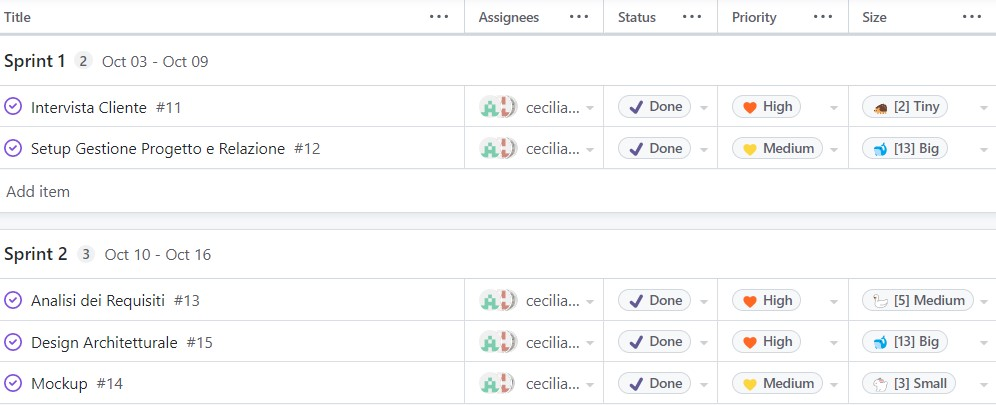
\includegraphics[width=\textwidth]{process/Img/sprint1_2.jpg}
    \label{fig:Sprint1_2}
\end{figure}
\begin{figure}[H]
    \centering
    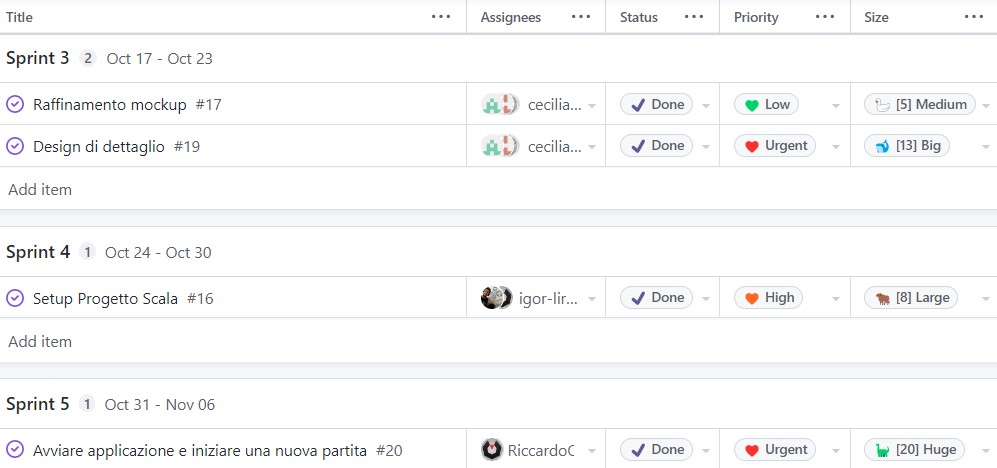
\includegraphics[width=\textwidth]{process/Img/sprint3_4_5.jpg}
    \label{fig:Sprint3_4_5}
\end{figure}
\begin{figure}[H]
    \centering
    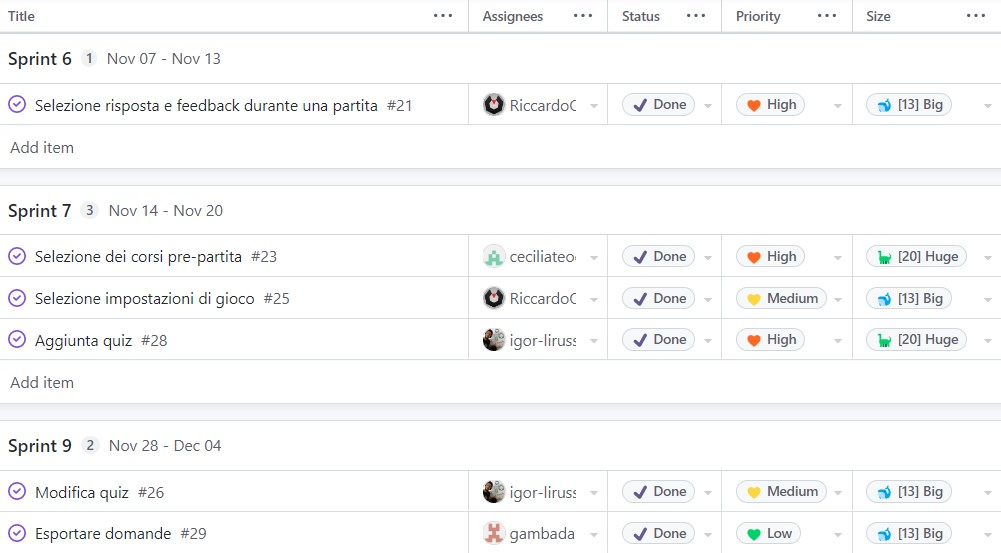
\includegraphics[width=\textwidth]{process/Img/sprint6_7_9.jpg}
    \label{fig:Sprint6_7_9}
\end{figure}
\begin{figure}[H]
    \centering
    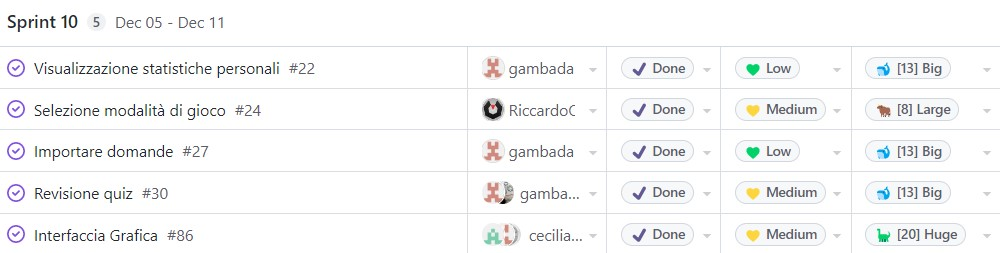
\includegraphics[width=\textwidth]{process/Img/sprint10.jpg}
    \label{fig:Sprint10}
\end{figure}

Nel capitolo finale \ref{chap:final-stats} sono invece inseriti dei grafici relativi al processo di sviluppo.
    
    \chapter{Sprint 1}
    \section{Sprint Goal}
        \section{Sprint Goal}
Durante questo primo sprint si è deciso come organizzare il team e come gestire il progetto:
\begin{itemize}
    \item Realizzare un'intervista con il committente con lo scopo di definire i requisiti del gioco
    \item Organizzare la relazione e la gestione del progetto
    \begin{itemize}
        \item Impostare la relazione e il progetto su GitHub
        \item Identificare gli elementi base del processo di sviluppo quali:
            \begin{itemize}
                \item Definition of done
                \item Durata degli sprint
                \item Quando e come effettuare i meetings
            \end{itemize}  
        \item Decidere quali strumenti/tool utilizzare:
            \begin{itemize}
                \item Applicativo per la creazione della relazione (Overleaf)
                \item Applicativo per la creazione di diagrammi (Miro)
                \item Bot Telegram per le eventuali notifiche riguardanti il repository
            \end{itemize}        
        \end{itemize}   
\end{itemize}

    \section{Sprint Backlog}
        %descrizione del refinement e immagine sprint backlog
Lo \href{https://github.com/orgs/ISIQuiz/projects/3/}{sprint backlog} risultante:
\begin{figure}[H]
    \centering
    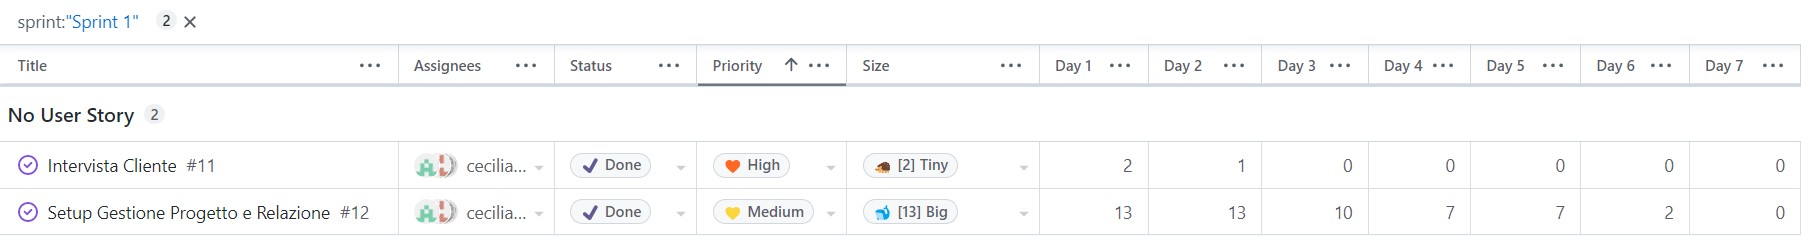
\includegraphics[width=\textwidth]{process/Img/Sprint1BL.jpg}
    \caption{Sprint 1 backlog}
    \label{fig:Sprint1}
\end{figure}


    \section{Sprint Review}
        \section{Sprint 1 Review}
%only this part is present also in the main report
Durante questo primo sprint abbiamo completato l'organizzazione di massima.
\paragraph{Deliverables} 
I deliverables per questo sprint sono stati i seguenti:
\begin{itemize}
    \item Intervista con il cliente corredata da domande
    \item Ubiquitous Language
    \item Setup Organizzazione GitHub
    \item Setup Report, con relativa repository e CI
\end{itemize}

    \section{Sprint Retrospective}
        Il primo sprint è stato svolto senza particolari problemi. Tutti i membri del gruppo hanno concordato sulle tecnologie e sugli strumenti da usare. L'Intervista con il cliente è stata svolta senza intoppi.


    
    \chapter{Sprint 2}
    \section{Sprint Goal}
        \section{Sprint Goal}
L'obiettivo dello sprint 2 è quello di effettuare l'analisi dei requisiti a partire dall'intervista effettuata precedentemente con l'esperto del dominio, ideare il design generale architetturale e realizzare una prima versione dei mockup da sottoporre poi al committente per avere un riscontro da tenere in considerazione per eventuali modifiche.

    \section{Sprint Backlog}
        %descrizione del refinement e immagine sprint backlog
Lo \href{https://github.com/orgs/ISIQuiz/projects/3/views/13}{sprint backlog} risultante:
\begin{figure}[H]
    \centering
    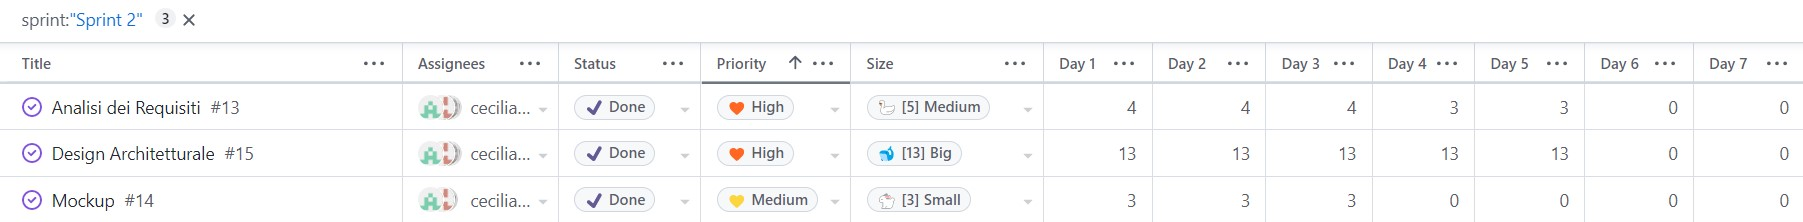
\includegraphics[width=\textwidth]{process/Img/Sprint2BL.jpg}
    \caption{Sprint 2 backlog}
    \label{fig:Sprint2}
\end{figure}

    \section{Sprint Review}
        \section{Sprint 2 Review}
%only this part is present also in the main report
Durante questo sprint abbiamo realizzato l'analisi dei requisiti del sistema e ideata l'architettura generale del sistema, dalla quale sono sorti alcuni dubbi che sono stati poi discussi e chiariti con l'esperto del dominio. Sono state realizzare due versioni dei mockup dell'applicazione, le quali hanno ricevuto entrambe giudizi positivi, ma andranno successivamente unite e raffinate per soddisfare al meglio i requisiti del committente.
\paragraph{Deliverables} 
I deliverables per questo sprint sono stati i seguenti:
\begin{itemize}
    \item Mockup
    \item Diagramma dei casi d'uso
    \item Diagramma delle classi
\end{itemize}

    \section{Sprint Retrospective}
        \section{Sprint Retrospective}
Durante il secondo sprint ci sono stati diversi momenti in cui il team si è trovato a dover riflettere su alcuni aspetti che risultavano poco chiari o che non erano stati adeguatamente approfonditi durante l'intervista con l'esperto del dominio. Questo è avvenuto soprattutto durante l'analisi dei requisiti e il design generale dell'architettura. A seguito del confronto eseguito durante uno dei meeting, è stato ritenuto che tali aspetti sono stati chiariti.
    
    \chapter{Sprint 3}
    \section{Sprint Goal}
        Sprint Goal

    \section{Sprint Backlog}
        %descrizione del refinement e immagine sprint backlog
In questo sprint il refinement è iniziato ad essere più accurato, essendo la parte organizzativa volta quasi al termine. Il refinement è stato svolto incrementalmente e ha scomposto il design principale in più sotto-issue, ognuna corrispondente al model, alla view e al controller. Il raffinamento dei mockup è stato scomposto nel raffinamento di ogni schermata.  Infine, la userstory è stata scomposta nell avvio di una partita, nella creazione della pagina principale e nella creazione del meccanismo di domanda e risposta. 

Lo \href{https://github.com/orgs/ISIQuiz/projects/3/}{sprint backlog} risultante:

\begin{figure}[H]
    \centering
    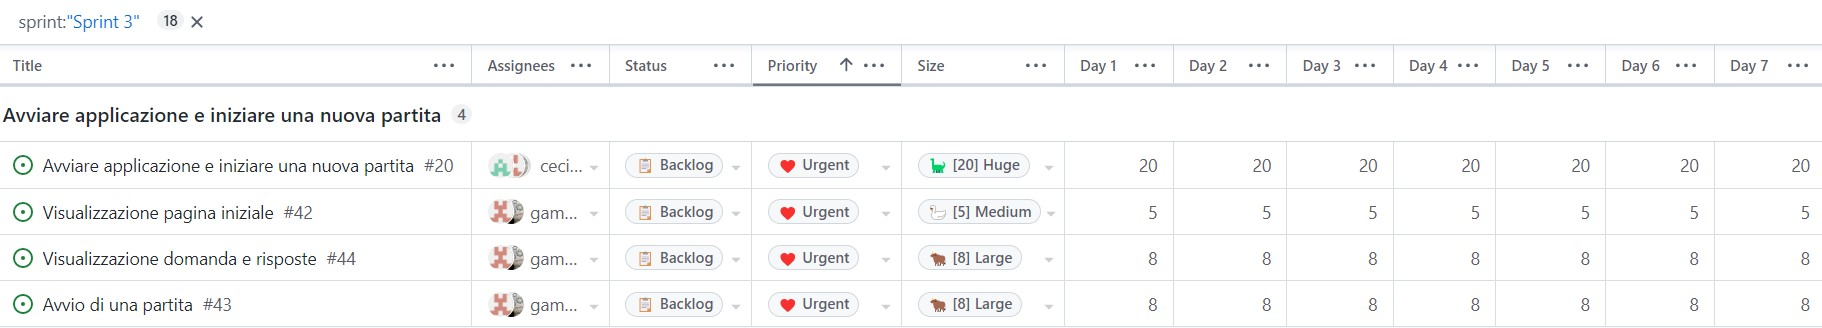
\includegraphics[width=\textwidth]{process/Img/Sprint3BL1.jpg}
    \label{fig:Sprint3BL1}
\end{figure}
\begin{figure}[H]
    \centering
    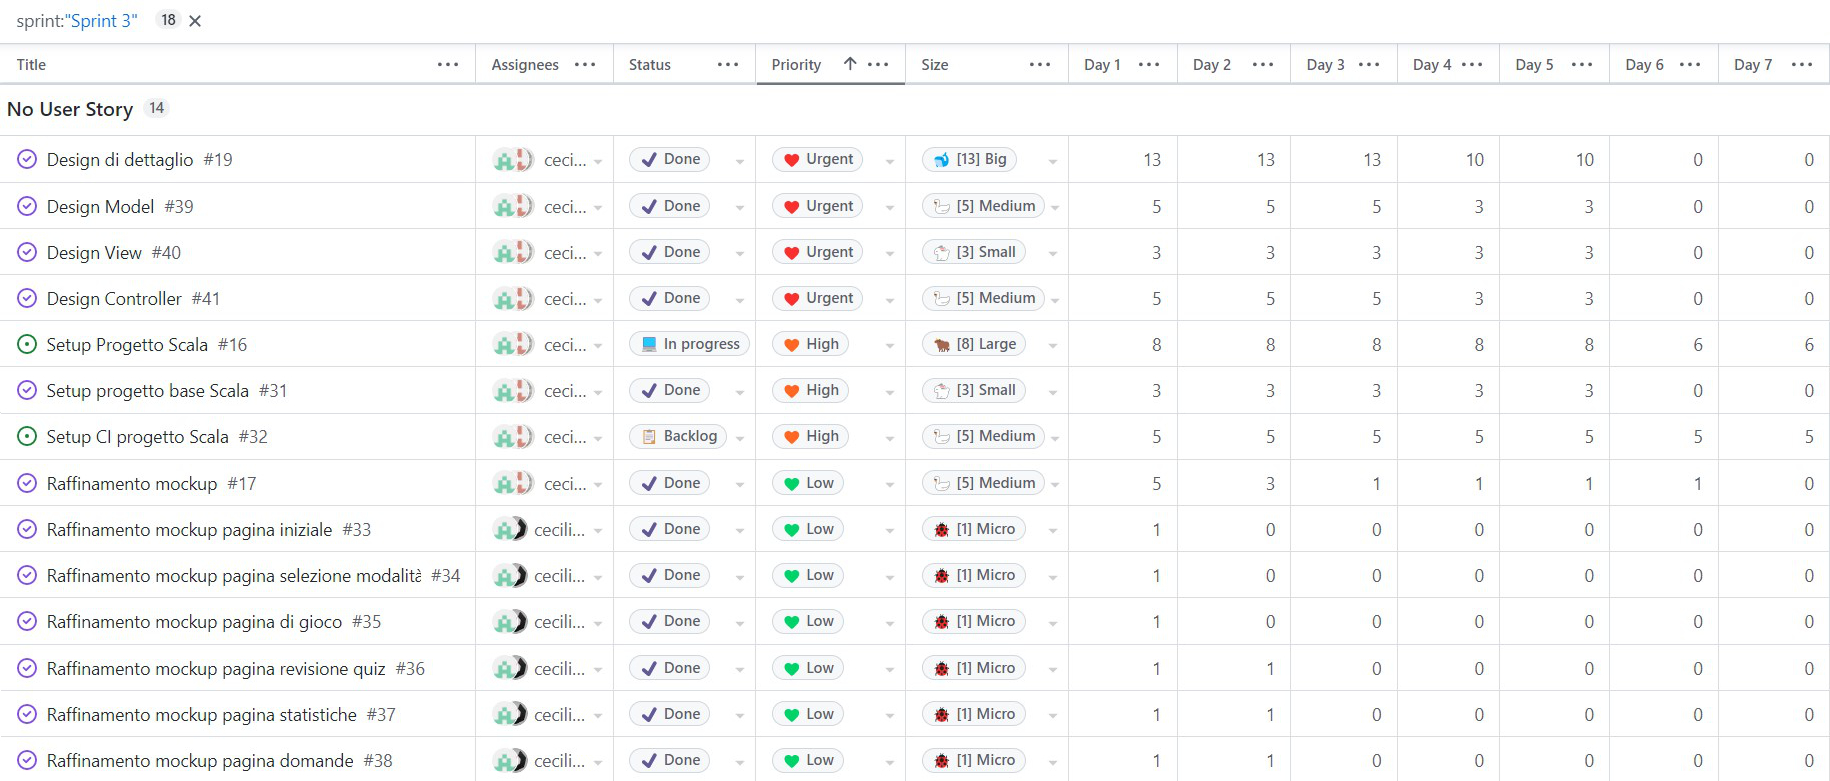
\includegraphics[width=\textwidth]{process/Img/Sprint3BL2.jpg}
    \label{fig:Sprint3BL2}
    \caption{Sprint 3 backlog}
\end{figure}

    \section{Sprint Review}
        \section{Sprint 3 Review}
%only this part is present also in the main report
Abbiamo studiato/implementato...
\paragraph{Deliverables} 
obiettivi raggiunti
\begin{itemize}
    \item uno
    \item due
    \item tre
\end{itemize}

    \section{Sprint Retrospective}
        \section{Sprint Retrospective}
Sprint retrospective thoughts 
        
    \chapter{Sprint 4}
    \section{Sprint Goal}
        %Sprint Goal
L'obbiettivo di questo quarto sprint è quello di completare il setup della CI del progetto e di realizzare un applicativo base con interfaccia grafica a riga di comando che possa:
\begin{itemize}
    \item Avviare una nuova partita;
    \item Visualizzare pagina iniziale;
    \item Visualizzare una domanda e le relative risposte;
    \item Selezionare una risposta ed ottenere un feedback sulla correttezza della scelta.
\end{itemize} 



    \section{Sprint Backlog}
        %descrizione del refinement e immagine sprint backlog
    \section{Sprint Review}
        %only this part is present also in the main report.
Durante questo sprint è stata implementata completamente la visualizzazione della pagina iniziale, è stata implementata la risposta di un quiz ed è stato effettuato il setup della CI.
\paragraph{Deliverables} 
I deliverables per questo sprint sono stati i seguenti:
\begin{itemize}
    \item Visualizzazione della pagina iniziale
    \item Implementata risposta di un quiz
    \item Setup della CI 
\end{itemize}

    \section{Sprint Retrospective}
        %Sprint retrospective thoughts 
        
    \chapter{Sprint 5}
    \section{Sprint Goal}
        L'obbiettivo di questo quinto sprint è quello di completare l'avvio di una partita, completare la visualizzazione di una una domanda e ottenere un feedback una volta scelta la risposta:
\begin{itemize}
    \item Avviare una nuova partita;
    \item Visualizzare una domanda;
    \item Selezionare una risposta ed ottenere un feedback sulla correttezza della scelta.
\end{itemize} 



    \section{Sprint Backlog}
        %descrizione del refinement e immagine sprint backlog

Lo \href{https://github.com/orgs/ISIQuiz/projects/3/views/16}{sprint backlog} risultante:

\begin{figure}[H]
    \centering
    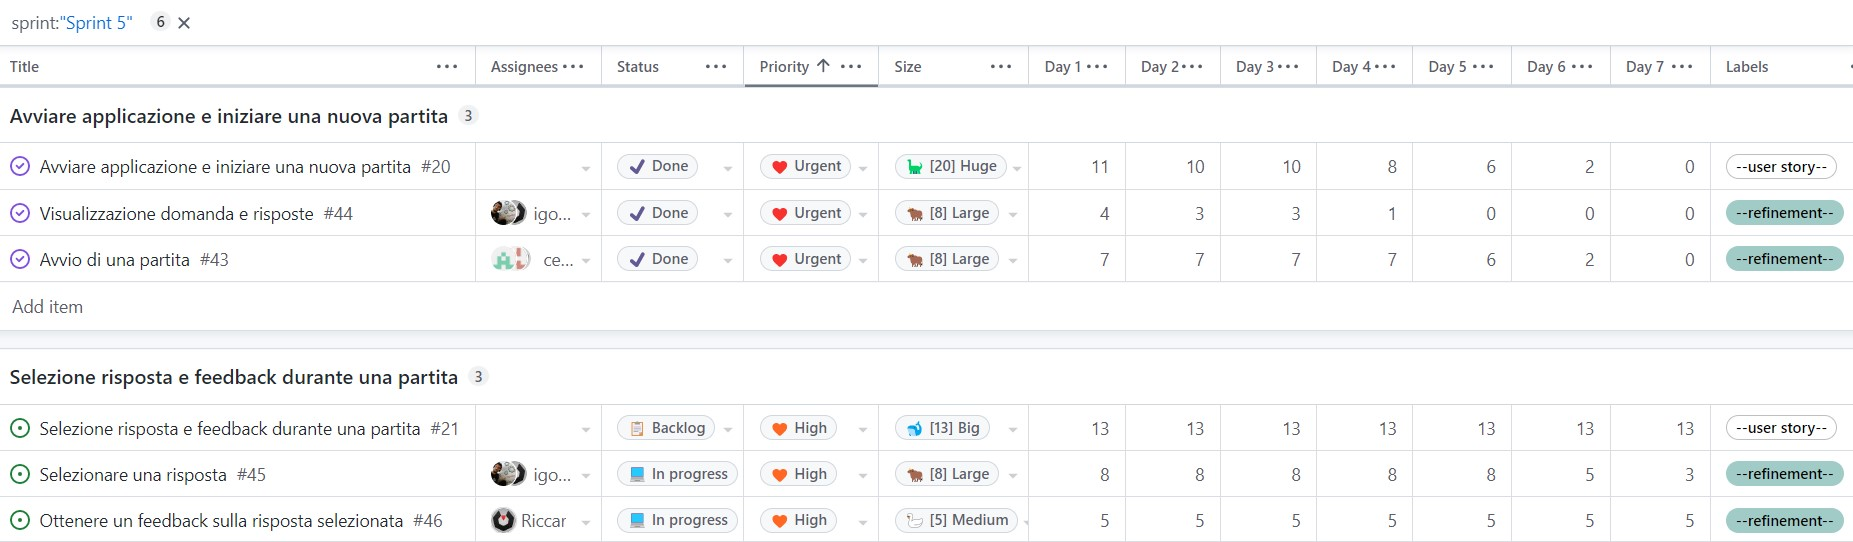
\includegraphics[width=\textwidth]{process/Img/Sprint5BL.jpg}
    \label{fig:Sprint5BL}
\end{figure}
    \section{Sprint Review}
        %only this part is present also in the main report.
Durante questo sprint abbiamo sviluppato la possibilità di avviare una partita tramite utilizzando il menu principale, inoltre è stata implementata la visualizzazione delle domande e delle rispettive risposte.
\paragraph{Deliverables} 
I deliverables per questo sprint sono stati i seguenti:
\begin{itemize}
    \item Avvio di una partita;
    \item Navigazione del menu principale;
    \item Visualizzazione domande e risposte.
\end{itemize}

    \section{Sprint Retrospective}
        Lo sprint ha prodotto risultati soddisfacenti. Un'unica nota, emersa durante lo sviluppo, è che la sovrapposizione di alcuni compiti ha reso viscosa e difficilmente parallelizzabile l'implementazione tra i membri del team. Individuato il problema, è stato scelto di raffinare con molta più cura le user stories, creando task più piccoli. Questo ci permette di fare merge con il branch di development molto più spesso, abilitando gli altri membri del team ad utilizzare gli elementi sviluppati per progredire con altre funzioni dipendenti da essi.
        
    \chapter{Sprint 6}
    \section{Sprint Goal}
        %Sprint Goal
L'obbiettivo di questo sprint è quello di rendere giocabile il programma, finendo di sviluppare la versione base. Questo comprende:
\begin{itemize}
    \item Selezionare le risposte e ottenere dei feedback
    \item Selezione dei corsi pre-partita
    \item Aggiunta domande
\end{itemize} 
    \section{Sprint Backlog}
        %descrizione del refinement e immagine sprint backlog

Lo \href{https://github.com/orgs/ISIQuiz/projects/3/views/17}{sprint backlog} risultante:

\begin{figure}[H]
    \centering
    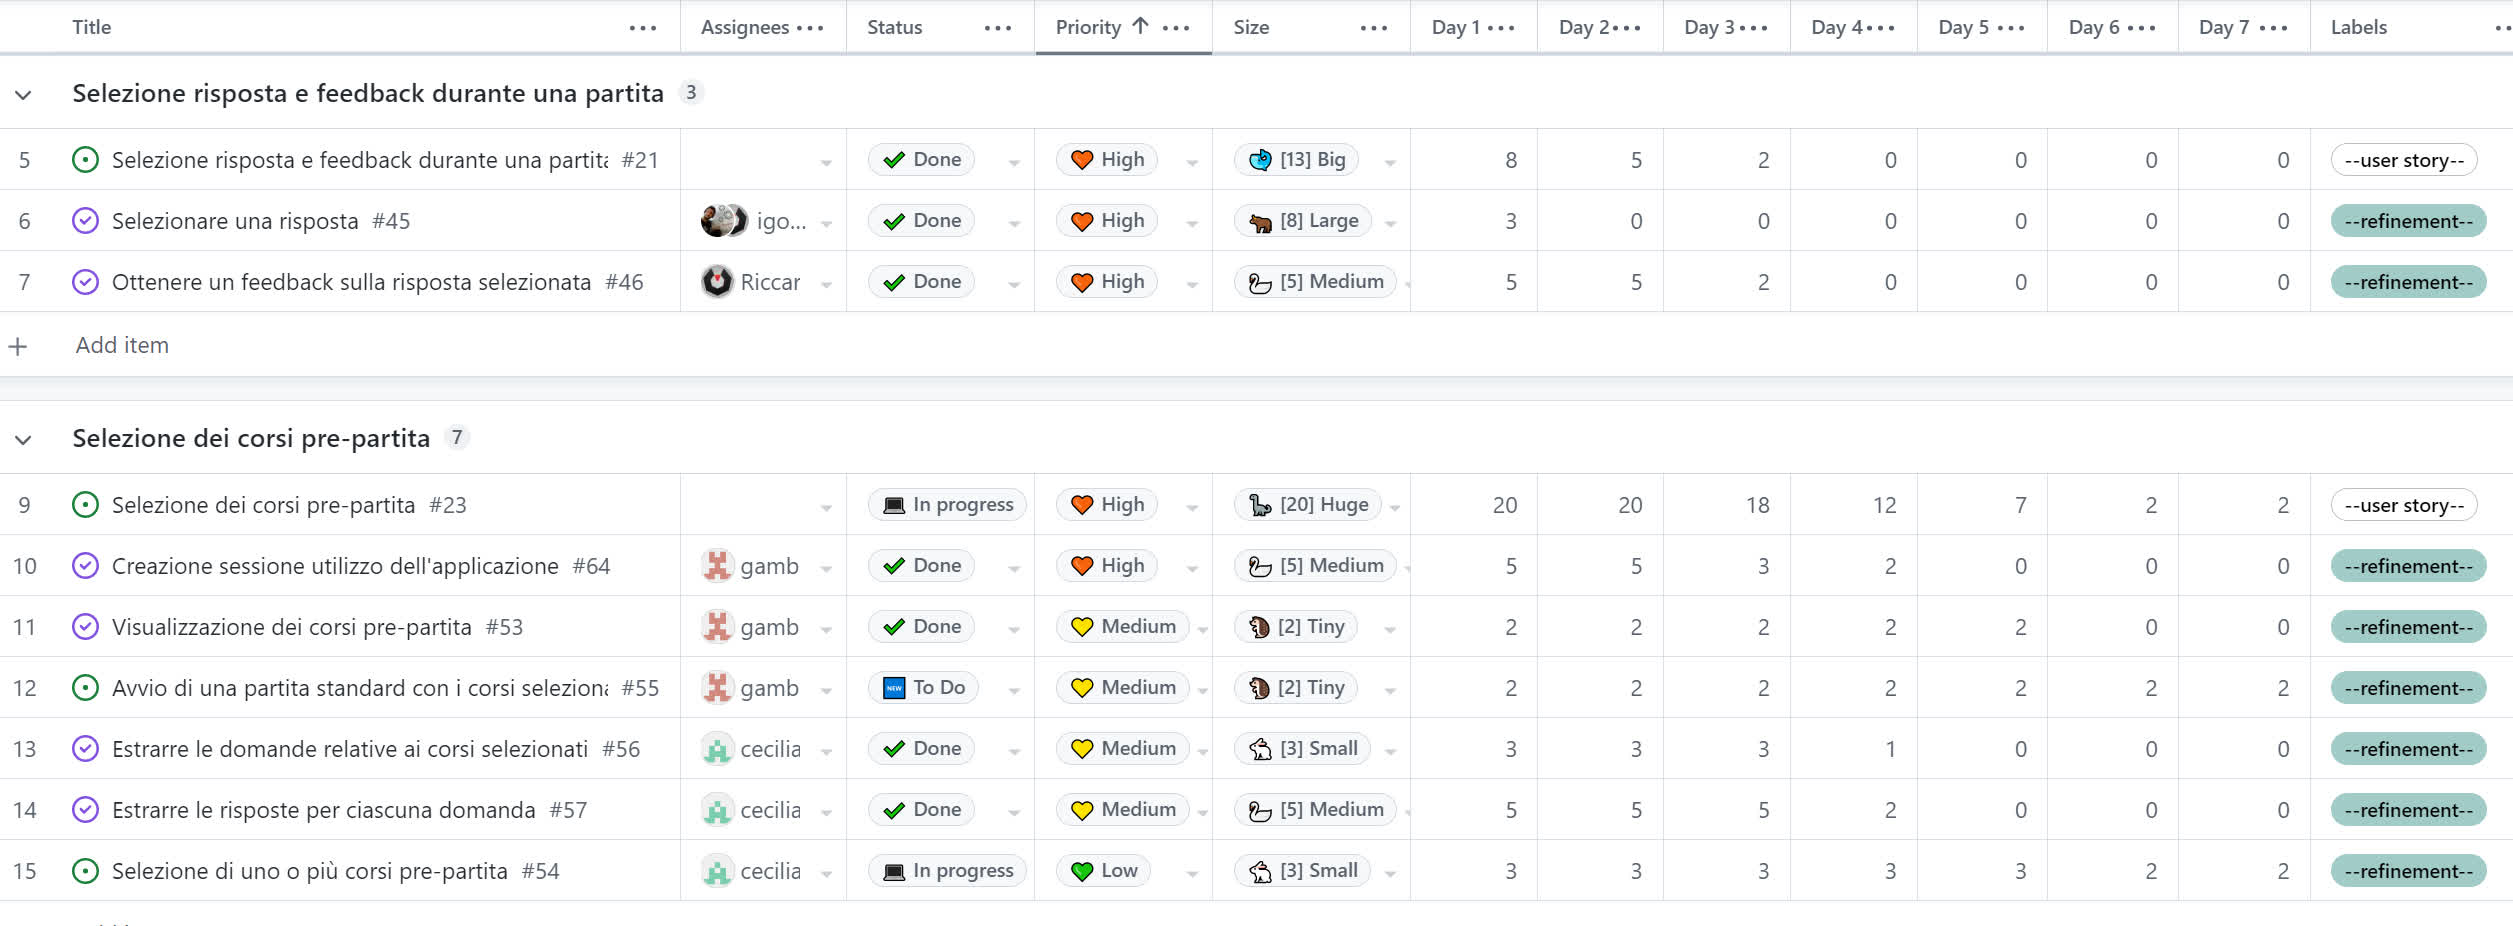
\includegraphics[width=\textwidth]{process/Img/Sprint6BL1.jpg}
    \label{fig:Sprint6BL1}
\end{figure}
\begin{figure}[H]
    \centering
    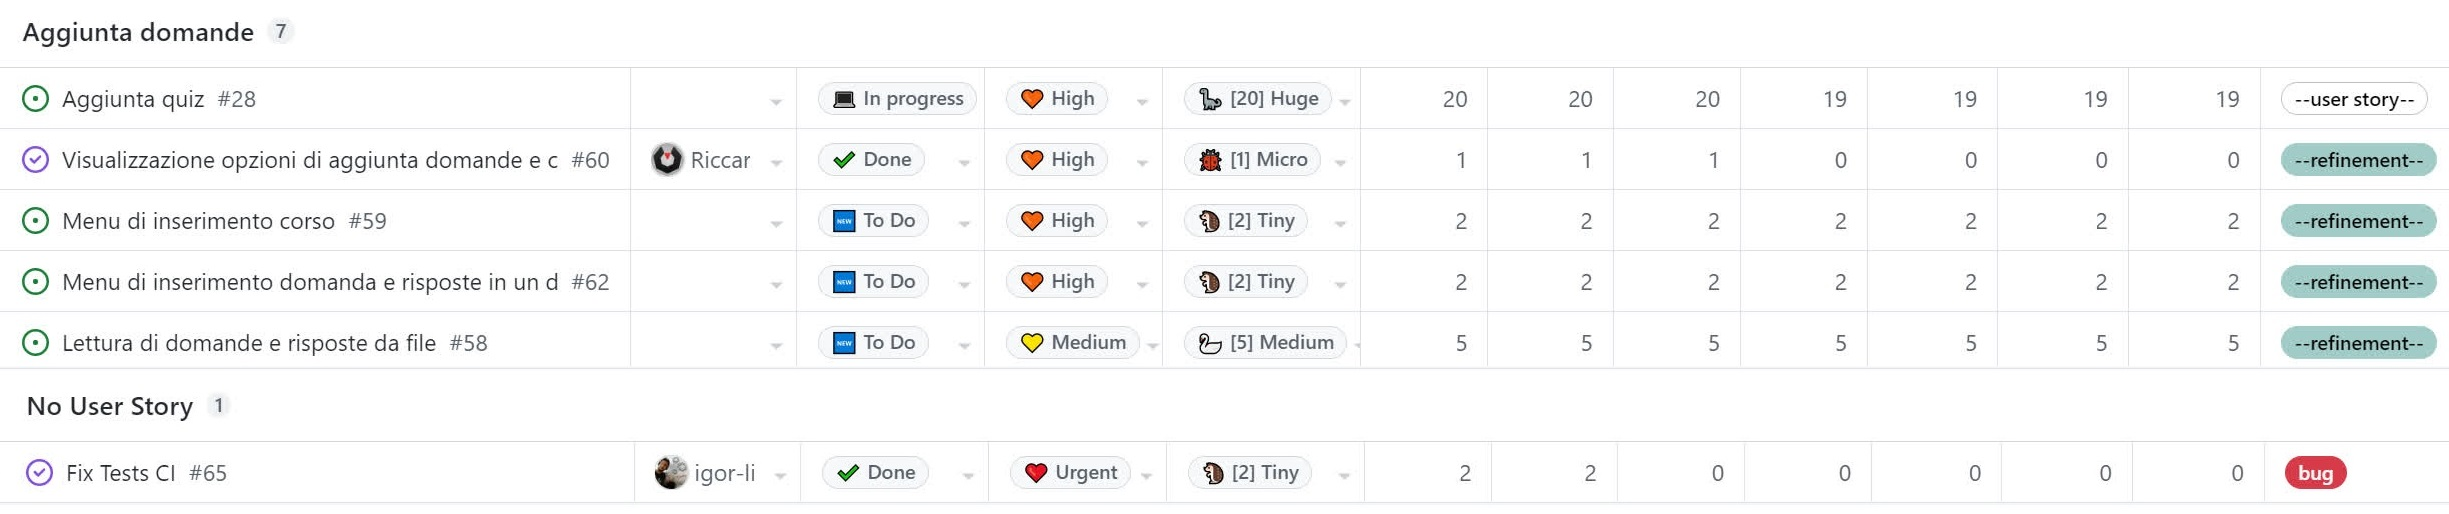
\includegraphics[width=\textwidth]{process/Img/Sprint6BL2.jpg}
    \label{fig:Sprint6BL2}
\end{figure}


    \section{Sprint Review}
        %only this part is present also in the main report.
Durante questo sprint sono stati implementati i meccanismi di selezione risposta e feedback su di essa. Inoltre, sono ora visibili e selezionabili i corsi disponibili prima di iniziare una partita e le domande relative ad esse sono estratte dal pool generale di quiz. Per ogni domanda inoltre, per variare l'esperienza, sono anche estratte a sorte varie possibili risposte. La sessione di ogni utente è ora salvata. Infine, è stato corretto il setup della CI.
\paragraph{Deliverables} 
I deliverables per questo sprint sono stati i seguenti:
\begin{itemize}
    \item Selezionare le risposte e ottenere dei feedback
    \item Selezione dei corsi pre-partita
    \item Visualizzazione delle opzioni di aggiunta domande
    \item Test automatici nella CI GitHub
\end{itemize}

    \section{Sprint Retrospective}
        Durante questo sprint, il carico di lavoro di ogni singolo componente è stato correttamente bilanciato e suddiviso. In questo modo, non essendoci sovrapposizioni, è stato più semplice portare a termine i task individuati indipendentemente dagli altri.
        
    \chapter{Sprint 7}
    \section{Sprint Goal}
        %Sprint Goal
L'obbiettivo di questo sprint è quello di completare la selezione dei corsi ed avviare una partita con quelli scelti, implementare la possibilità di aggiungere domande dalla view e da file, infine aggiungere la possibilità di selezionare le impostazioni di gioco. 
Questo comprende:
\begin{itemize}
    \item Completare la selezione dei corsi pre-partita
    \item Aggiunta domande
    \item Selezione impostazioni di gioco
\end{itemize} 
    \section{Sprint Backlog}
        %descrizione del refinement e immagine sprint backlog

Lo \href{https://github.com/orgs/ISIQuiz/projects/3/}{sprint backlog} risultante:

\begin{figure}[H]
    \centering
    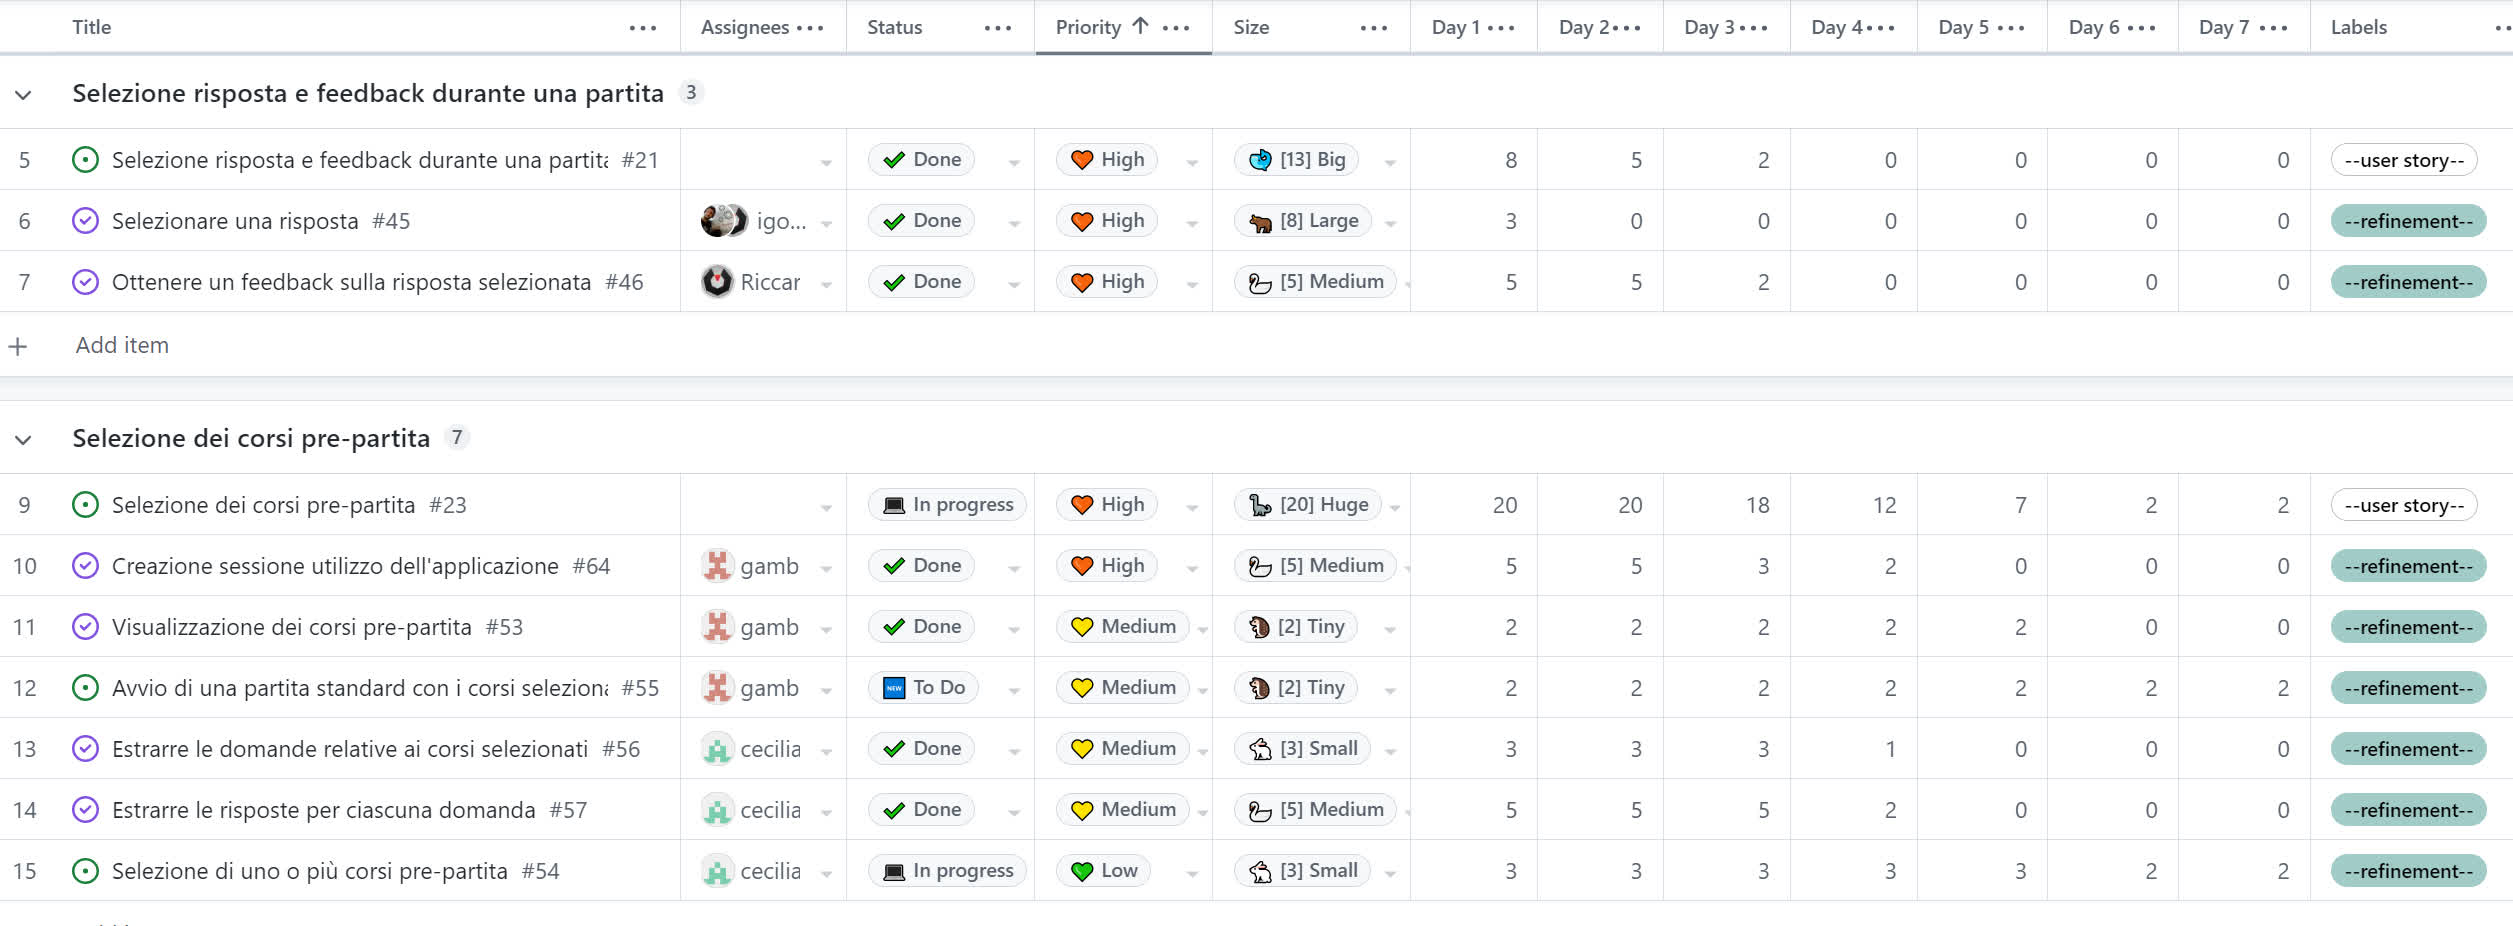
\includegraphics[width=\textwidth]{process/Img/Sprint6BL1.jpg}
    \label{fig:Sprint7BL}
\end{figure}
    \section{Sprint Review}
        %only this part is present also in the main report.
Durante questo sprint è stata implementata completamente la visualizzazione della pagina iniziale, è stata implementata la risposta di un quiz ed è stato effettuato il setup della CI.
\paragraph{Deliverables} 
I deliverables per questo sprint sono stati i seguenti:
\begin{itemize}
    \item Visualizzazione della pagina iniziale
    \item Implementata risposta di un quiz
    \item Setup della CI 
\end{itemize}

    \section{Sprint Retrospective}
        Non ci sono particolari aspetti da evidenziare riguardo allo svolgimento di questo sprint in quanto, come già detto, tutti i task sono stati suddivisi correttamente e portati a termine dal team.
        
    \chapter{Sprint 8}
    \section{Sprint Goal}
        %Sprint Goal
L'obbiettivo di questo sprint è quello di completare la partita e rivedere i quiz giocati. Inoltre si vuole visualizzare le statistiche personali proprie del giocatore. 
Infine in questo sprint si vuole implementare l'interfaccia grafica dell'applicazione, funzionante in parallelo con la linea di comando.
\begin{itemize}
    \item Visualizzazione risposta corretta per ogni quiz della partita
    \item Revisione quiz a fine partita
    \item Interfaccia grafica
\end{itemize} 
    \section{Sprint Backlog}
        %descrizione del refinement e immagine sprint backlog

Lo \href{https://github.com/orgs/ISIQuiz/projects/3/views/19}{sprint backlog} risultante:

\begin{figure}[H]
    \centering
    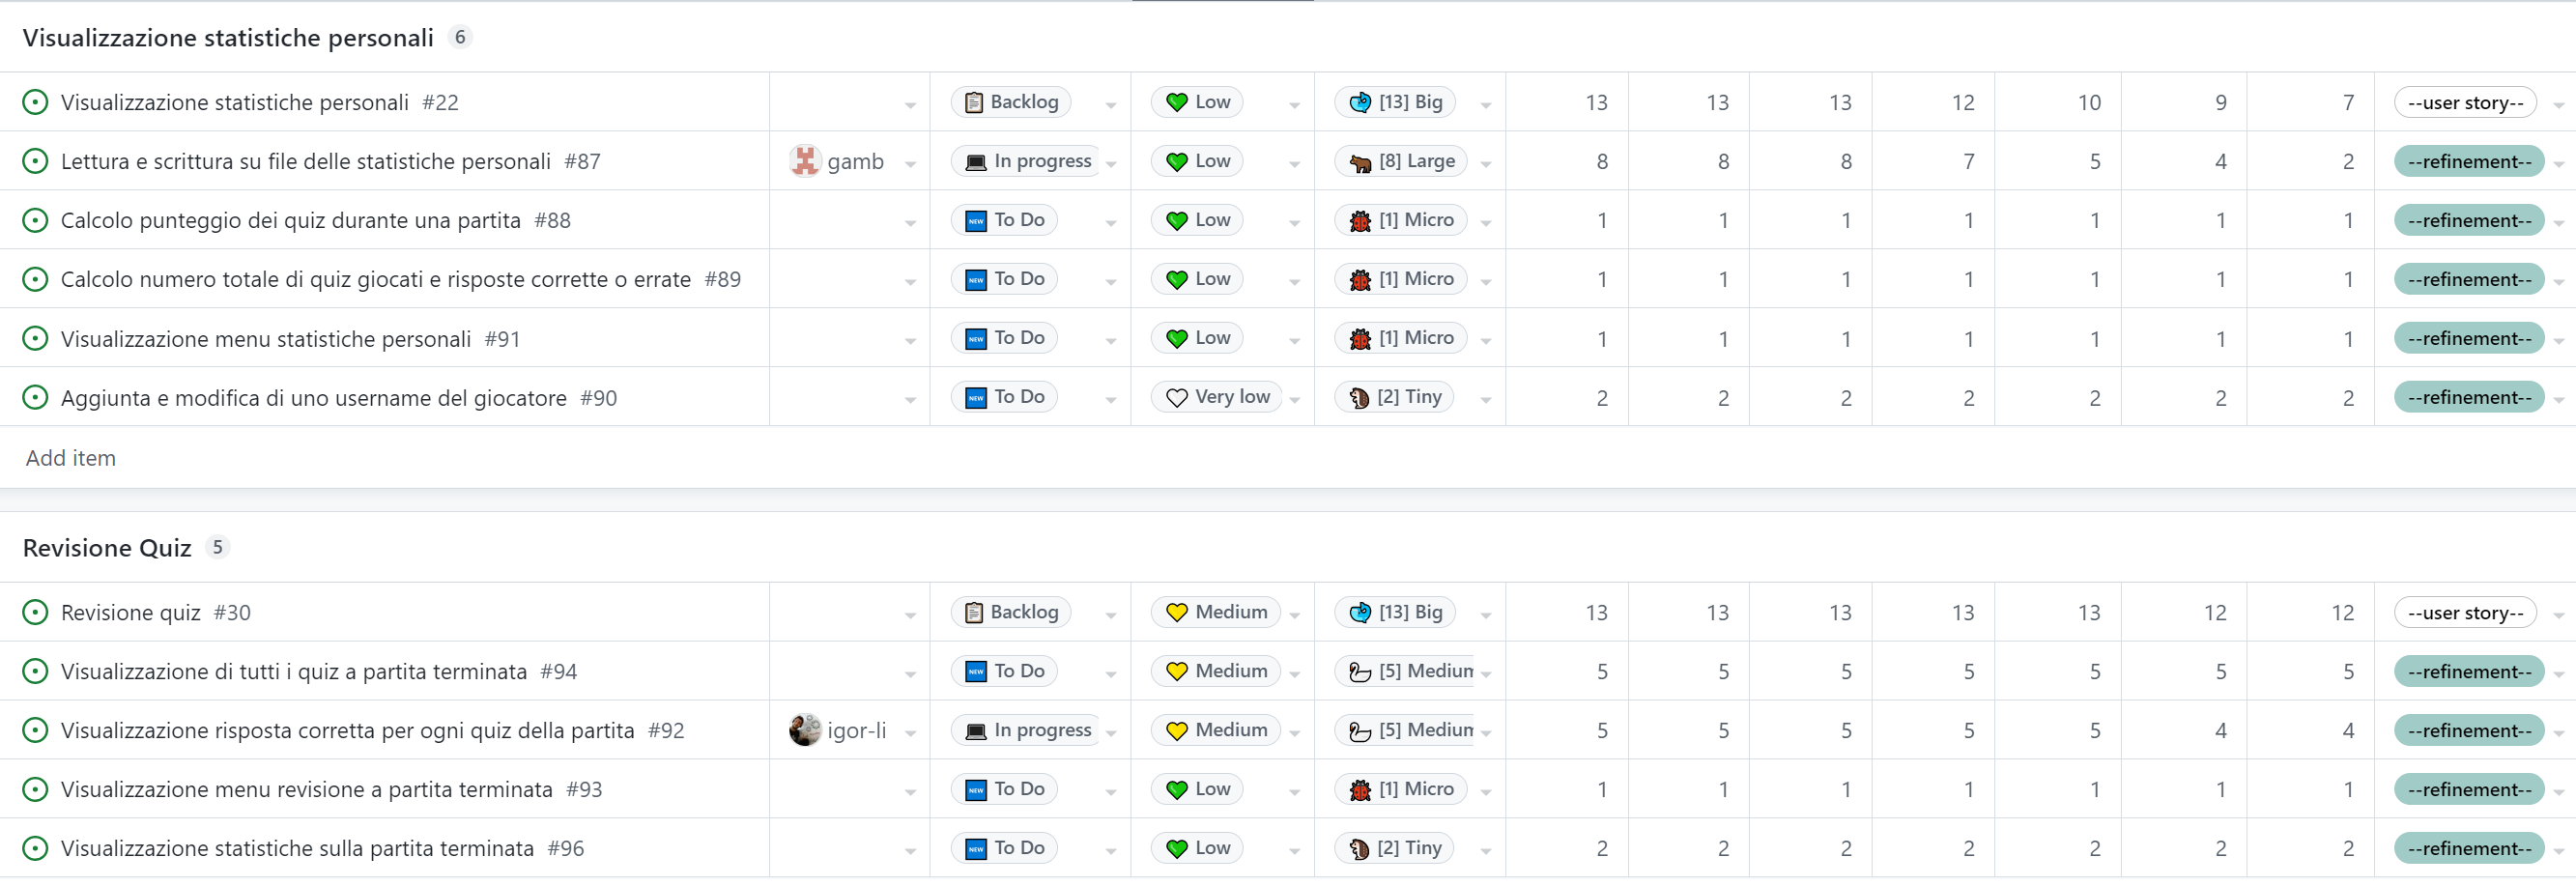
\includegraphics[width=\textwidth]{process/Img/Sprint8BL1.png}
    \label{fig:Sprint8BL}
\end{figure}

\begin{figure}[H]
    \centering
    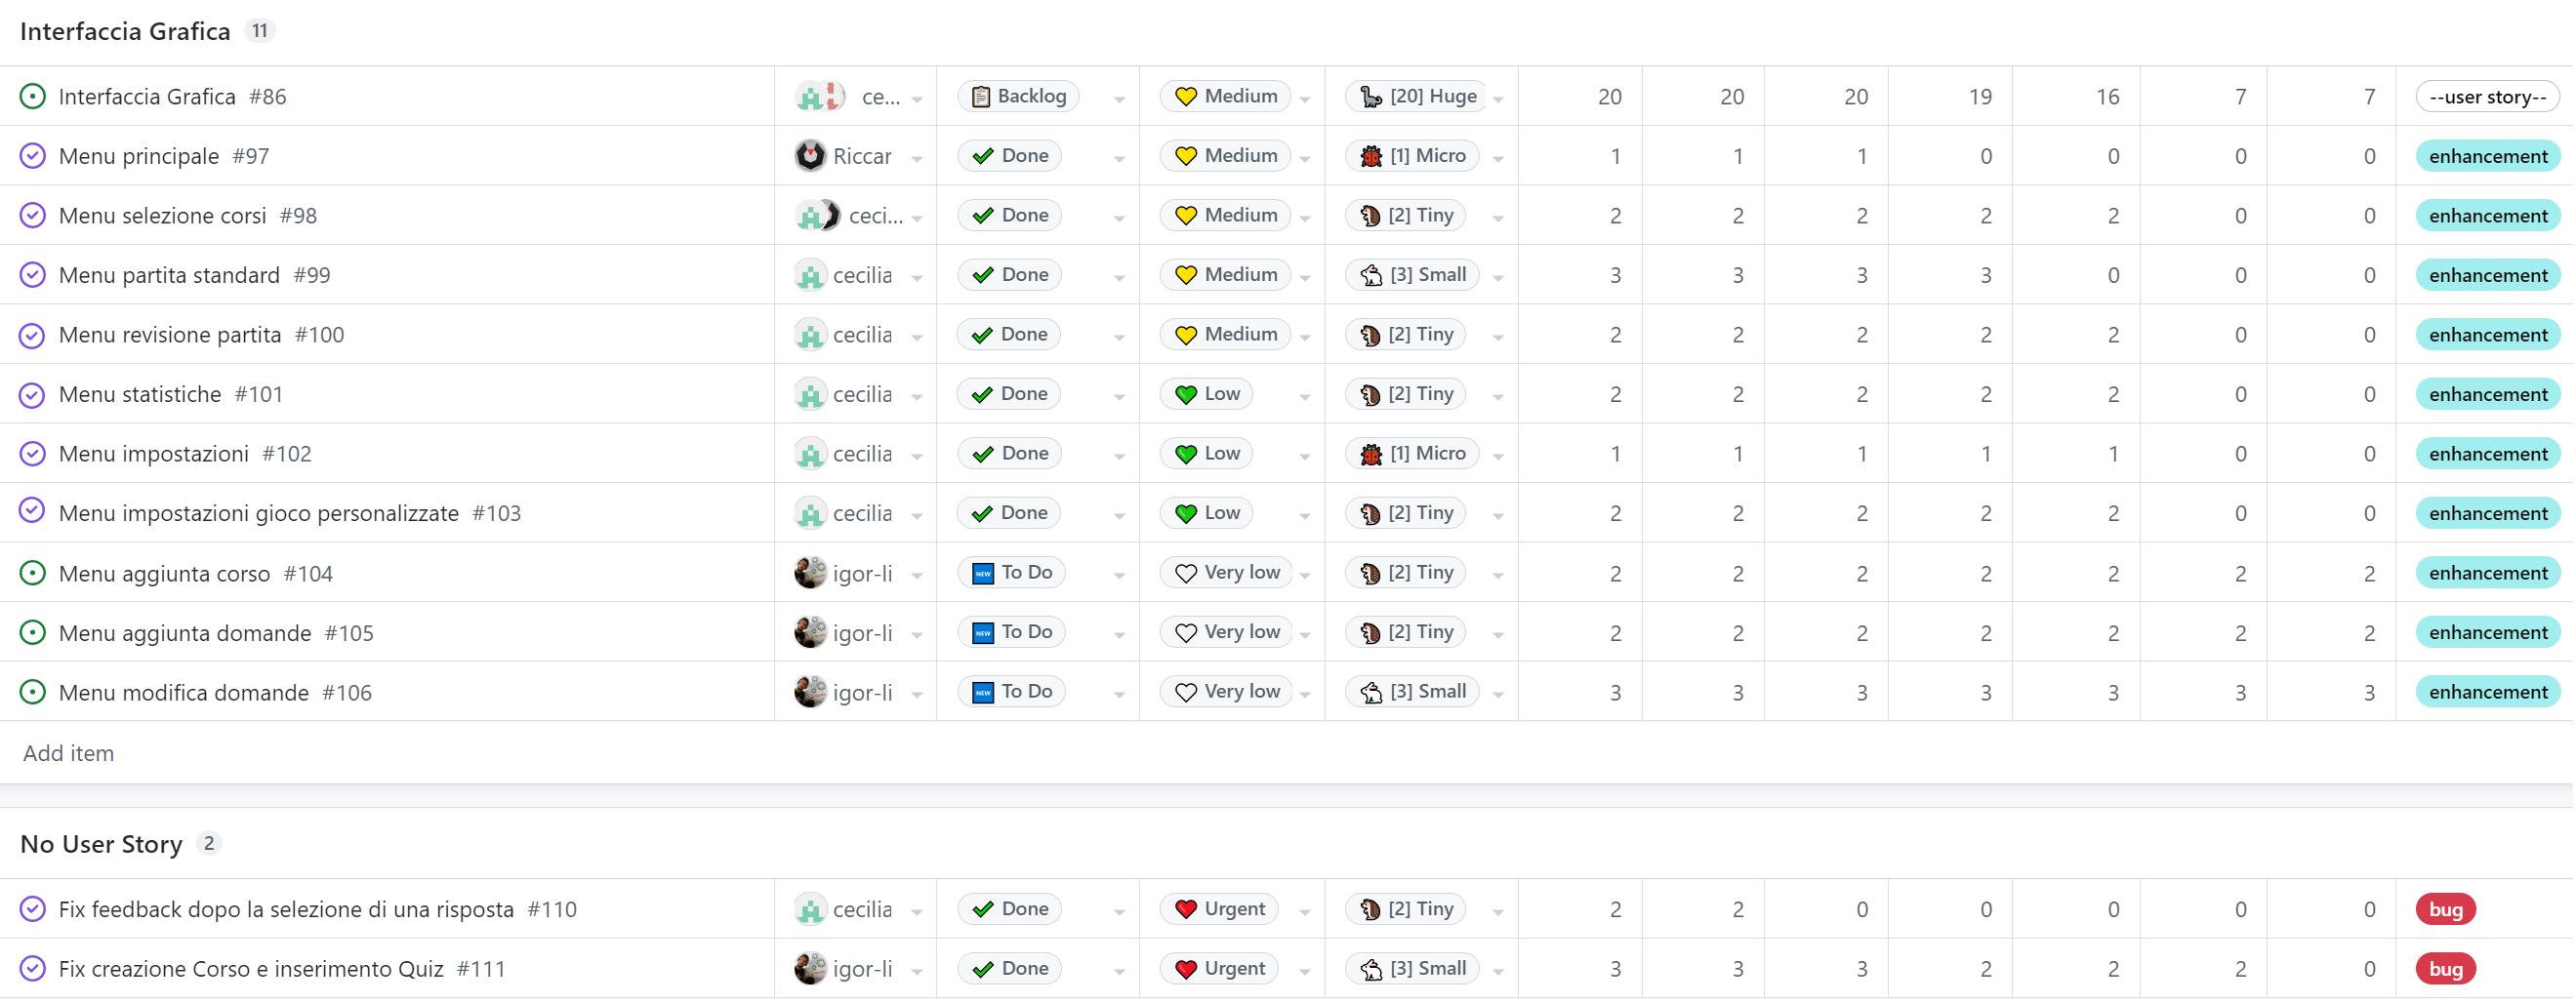
\includegraphics[width=\textwidth]{process/Img/Sprint8BL2.png}
    \label{fig:Sprint8BL}
\end{figure}
    \section{Sprint Review}
        %only this part is present also in the main report.
In questo sprint non sono stati completati tutti i goal a causa dei problemi che sono sorti principalmente durante l'aggiunta dell'interfaccia grafica basata su ScalaFX. Questo ha portato a diverse problematiche di compatibilità con la parte di interfaccia grafica da linea di comando precedentemente implementata.
\paragraph{Deliverables} 
I deliverables per questo sprint sono stati i seguenti:
\begin{itemize}
    \item Create schermate dell'applicazione in FXML
    \item Aggiunta navigazione tra le pagine tramite interfaccia grafica
\end{itemize}
    \section{Sprint Retrospective}
        A causa dei problemi sopra citati, non c'è stata una corretta organizzazione all'interno del team e non è stato possibile lavorare parallelamente. Di conseguenza, una parte dei compiti verranno sposati allo sprint successivo.
        
    \chapter{Sprint 9}
    \section{Sprint Goal}
        L'obbiettivo di questo sprint è quello di completare i goal dello sprint precedente, quindi la visualizzazione delle statistiche personali parte della revisione dei quiz e l'interfaccia grafica. Inoltre l'obbiettivo è di implementare la possibilità di scegliere la modalità di gioco e modificare, importare ed esportare le domande di un corso.
\begin{itemize}
    \item Completare la visualizzazione delle statistiche
    \item completare la revisione dei quiz a fine partita
    \item Completare l'Interfaccia grafica
    \item Selezione modalità di gioco
    \item Modifica domande
    \item Importare domande
    \item Esportare domande
\end{itemize} 
    
    \chapter{Meetings}

\section{Meetings}
\begin{itemize}
    \item 06/10/2022
        \begin{itemize}
            \item Decisa organizzazione generale
            \item Creato repository
        \end{itemize}
    \item 10/10/2022
        \begin{itemize}
            \item Intervista al domain expert
            \item Stesura requisiti utente, funzionali e non funzionali
            \item Stabilita definition of done
            \item Stabilito metodo di definizione dei pesi relativi ai task
        \end{itemize}
    \item 15/10/2022
        \begin{itemize}
            \item Review requisiti
            \item Creazione digramma classi e casi d'uso
            \item Definizione Ubiquitous Language
            \item Aggiunta e revisione mockup
        \end{itemize}
    \item 17/10/2022
        \begin{itemize}
            \item Riguardato il diagramma dei casi d'uso
            \item Sviluppato User Stories
            \item Creata la board di GitHub Projects
            \item Aggiornata la board di GitHub Projects
            \item Aggiornato il Gantt su Jira in base alle User Stories scelte
            \item Definizione task per lo Sprint 3
        \end{itemize}
    \item 20/10/2022
        \begin{itemize}
            \item Review dei mockup
            \item Schema relazione tra le view dei mockup
            \item Schema iniziale Model-View-Controller
        \end{itemize}
        
\end{itemize}


    
    \chapter{Final Statistics}
Statistiche finali sullo sviluppo e andamento del progetto corredate da grafici e tabelle
Da notare che le user stories appaiono sul product backlog solo sullo sprint che le ha concluse, ma possono essere state iniziate in precedenza. (I.E. L'interfaccia grafica è stata iniziata nello sprint 8 ma conclusa solo nel 10. Poichè ad una user-story, non possono essere assegnati più sprint appare solo nel suddetto Sprint Backlog, ma i suoi refinement sono presenti anche negli altri)

\nocite{*} % Includes all references from the `references.bib` file

\end{document}
